\section{Abstract}

"Might of Timaert" is an indie 2d procedural RPG with tile graphics. Game engine is based on cellular automata with a "real time" (game tick/10 $us$) world simulation. Cellular world is connected 1024x1024 array of cells with torus topology. All the physics (zones, fluids, climate etc.) is simulated on ancilla arrays. All the world objects are dynamically linked to relevant cells. It is expected to subsequently have an order of $10^4$ individual active game objects. Menus, fights, quests and others player-game interactions are realised using finite automata world states.

Games references: $mount-and-blade, dwarf-fortress, caves-of-qud, Elona+, fear-and-hunger$

Contact email:  
\href{mailto:jirnyak@gmail.com}{jirnyak@gmail.com} 
Telegram: 
\href{https://t.me/mankobus}{\nolinkurl{@mankobus}}
 GitHub: 
\href{https://github.com/Jirnyak}{\nolinkurl{Jirnyak}}

\begin{figure}[H]
    \centering
    
\includegraphics[height=4.5cm]{images/witch.png}
    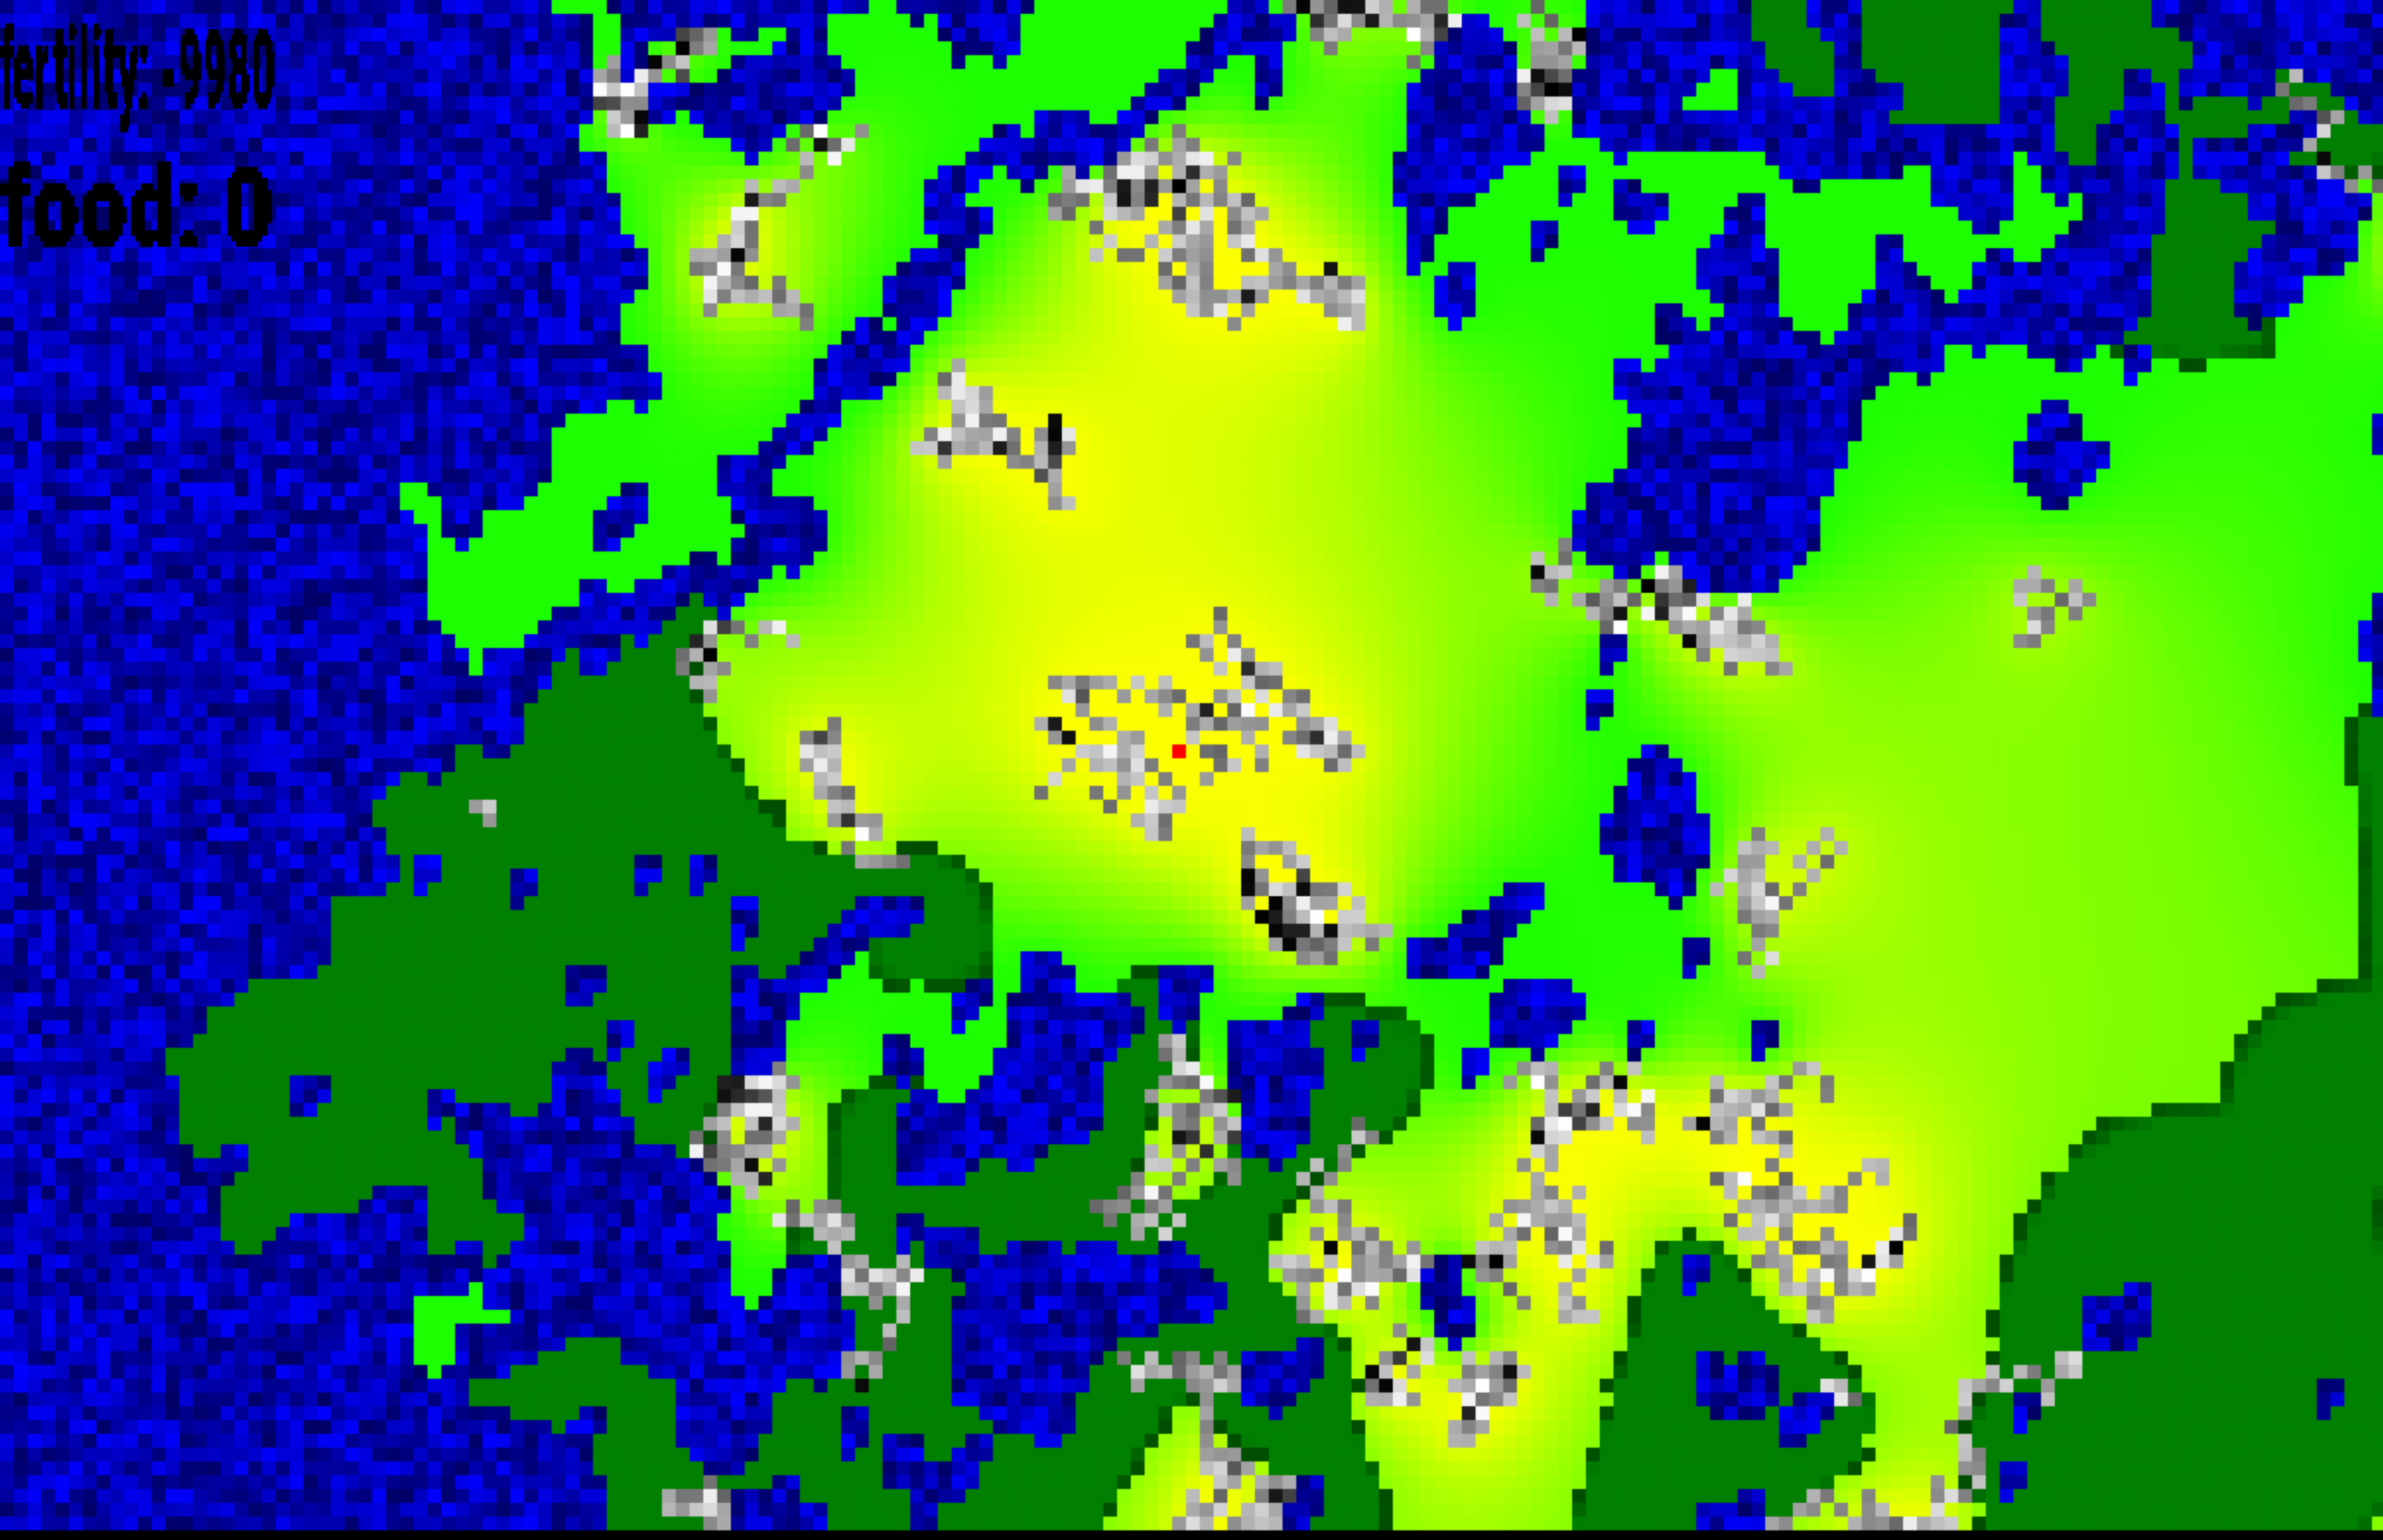
\includegraphics[height=4cm]{images/terrain.png}
    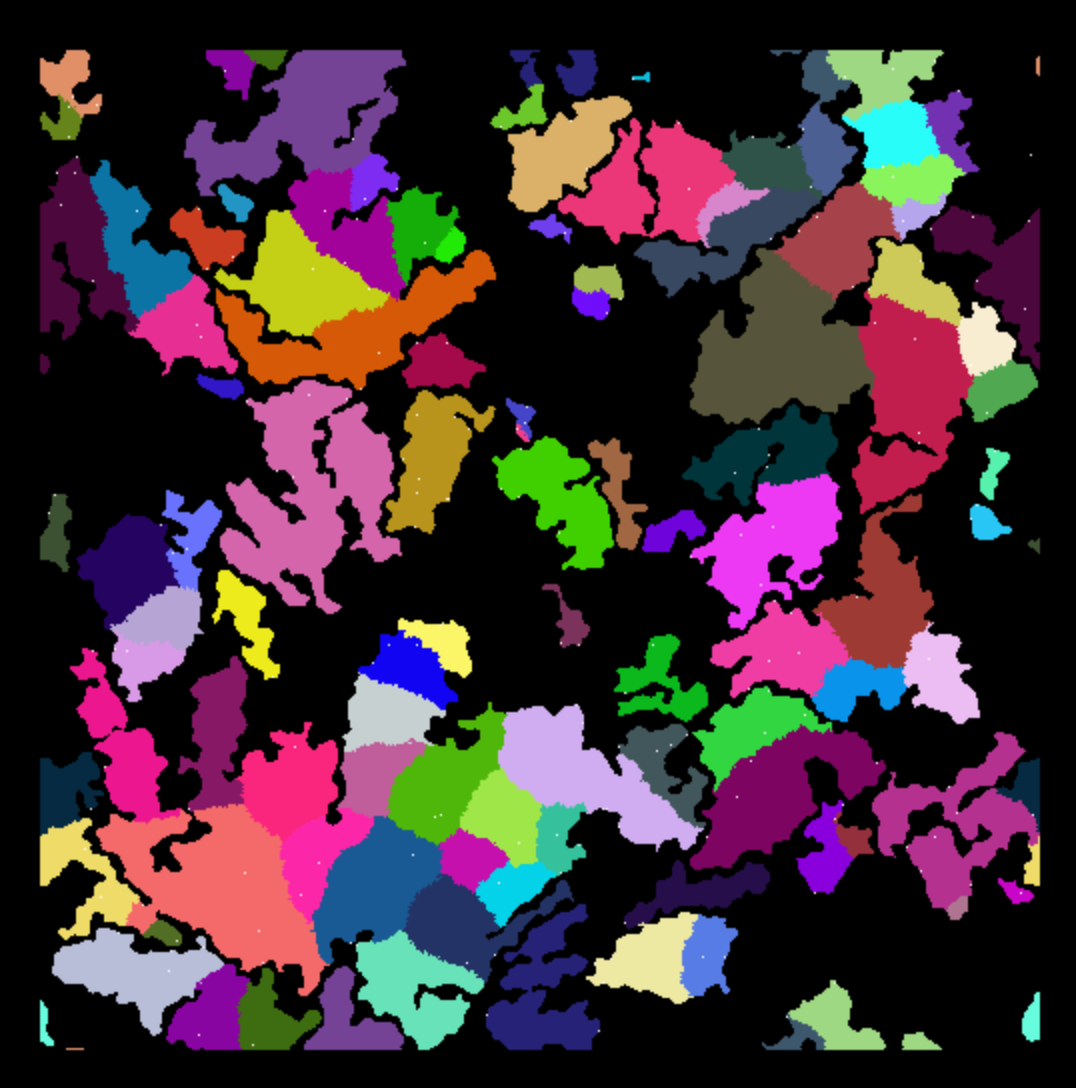
\includegraphics[height=4.5cm]{images/nations.png}
    \caption{1. An example of in game procedural quest.  2. An example of climatic zones. 3. An example of political map. Screenshots from game prototype.}
    \label{fig:witch}
\end{figure}

Download game prototype:
\href{https://drive.google.com/drive/folders/1TWdjQCXN2TFRXHNwMoggdR0XF6cGWThE?usp=sharing}{\nolinkurl{drive.google.com}}


\newpage

\tableofcontents

